%%%%%%%%%%%%%%%%%%%%%%%%%%%%%%%%%%%%%%%%%%%%
\section{Looking inside the human body}

%%%%%%%%%%%%%%%%%%%%%%%%%%%%%%%%%%%%%%%%%%%%%
%\subsection{FETUS}
%Medical imaging in pregnancy

%%%%%%%%%%%%%%%%%%%%%%%%%%%%%%%%%%%%%%%%%%%%%%%%%%%%%%%%
{
\paper{\url{https://en.wikipedia.org/wiki/Medical_imaging_in_pregnancy}}
\begin{frame}{Medical Imaging in Pregnancy}
      \begin{figure}
        \centering
        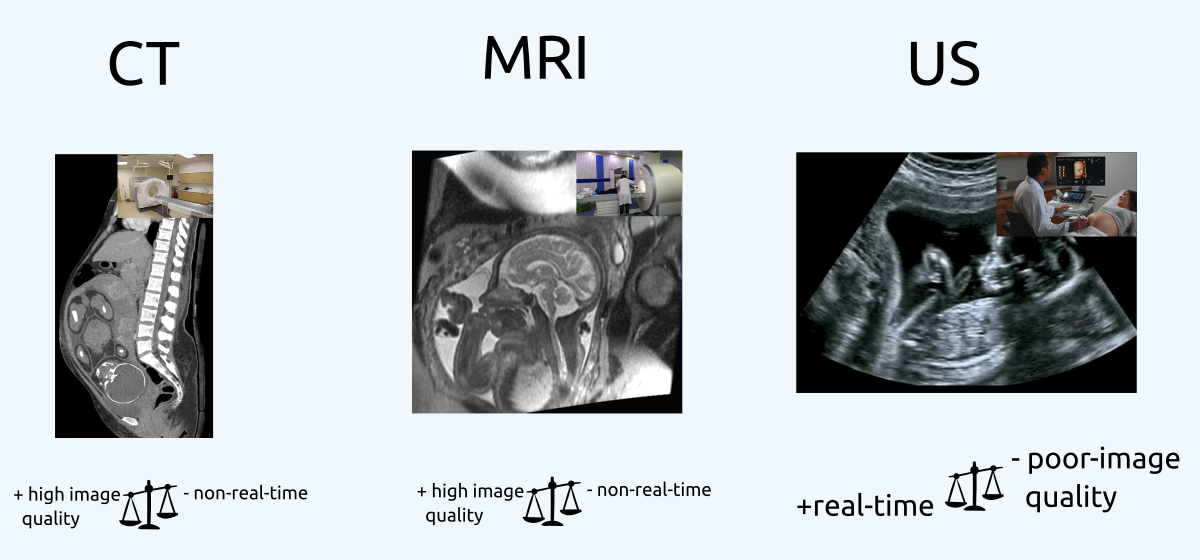
\includegraphics[width=1.0\textwidth]{./figures/medical-imaging/versions/drawing-v01.png}
        %\caption{}
      \end{figure}
\end{frame}
}


%%%%%%%%%%%%%%%%%%%%%%%%%%%%%%%%%%%%%%%%%%%%%%%%%%%%%%%%
{

\paper{Fetal and Mother Numerical Models (FEMONUM) in \url{http://femonum.telecom-paristech.fr}}
%https://perso.telecom-paristech.fr/angelini/projects_research/FEMONUM/femonum_en.html
%https://perso.telecom-paristech.fr/angelini/projects_research/FEMONUM/femonum_en.html

\begin{frame}{Modelling US imaging}
      \begin{figure}
        \centering
        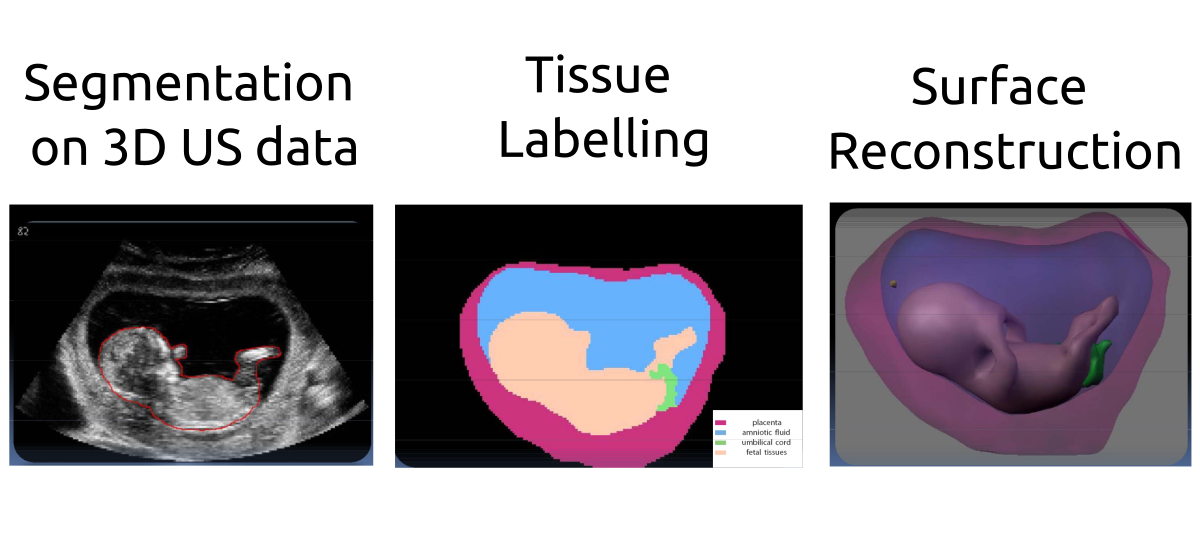
\includegraphics[width=1.0\textwidth]{./figures/modelling-us-imaging/versions/drawing-v01.png}
        %\caption{}
      \end{figure}
\end{frame}
}



%%%%%%%%%%%%%%%%%%%%%%%%%%%%%%%%%%%%%%%%%%%%%%%%%%%%%%%%
{
%\paper{3D printing FETUS}
\begin{frame}{3D printing FETUS}
      \begin{figure}
        \centering
        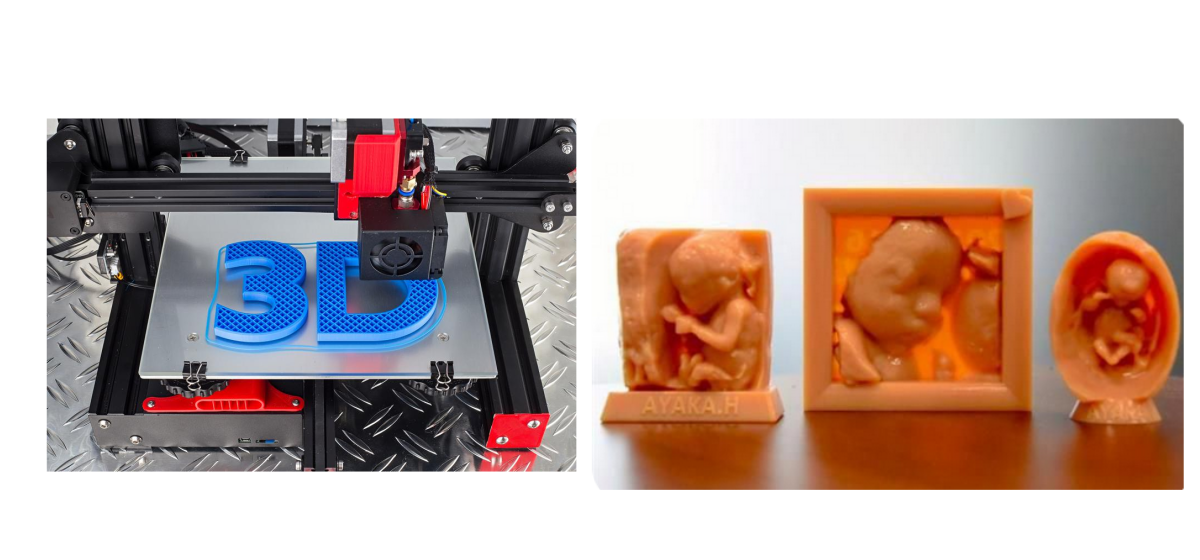
\includegraphics[width=1.0\textwidth]{./figures/3d-printing/versions/drawing-v00.png}
        %\caption{}
      \end{figure}
\end{frame}
}

%%%%%%%%%%%%%%%%%%%%%%%%%%%%%%%%%%%%%%%%%%%%%%%%%%%%%%%%
{
\begin{frame}
  \frametitle{Example 1}
  \vspace{10pt}
  \begin{center}
    \movie{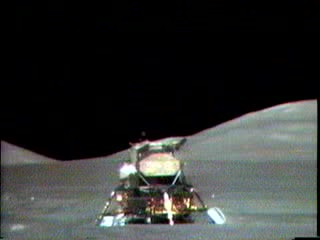
\includegraphics[width=0.5\textwidth]{./figures/apollo/apollo17.jpg}}{./figures/apollo/apollo17.avi}
  \end{center}

  \begin{itemize}
    \item Click on the image to play/pause the video.
    \item Move pointer to the bottom of the video frame for a draggable position
      control.
  \end{itemize}
\end{frame}
}
